\chapter{Задание \textnumero3}

В листинге~\ref{img:task03} приведён текст третьей программы.

\begin{lstlisting}[label=img:task03,caption={Текст третьей программы}]
#include <stdio.h>
#include <errno.h>
#include <stdlib.h>
#include <string.h>

int main(void)
{
    FILE *fss[2];
    const char alphabet[] = "Abcdefghijklmnopqrstuvwxyz";

    fss[0] = fopen("out.txt", "wr");
    if (!fss[0])
    {
        fprintf(stderr, "first fopen: %s\n", strerror(errno));
        exit(1);
    }
    fss[1] = fopen("out.txt", "wr");
    if (!fss[1])
    {
        fprintf(stderr, "second fopen: %s\n", strerror(errno));
        exit(1);
    }

    for (int i = 0; i < sizeof(alphabet)-1; ++i)
        fprintf(fss[i % 2], "%c", alphabet[i]);

    fclose(fss[0]);
    fclose(fss[1]);

    return 0;
}
\end{lstlisting}

На рисунке~\ref{img:task03} изображён результат работы третьей программы.

\begin{figure}[H]
    \includegraphics[scale=0.5]{images/task03.png}
    \caption{Результат работы третьей программы}\label{img:task03}
\end{figure}

В результате двух последовательных вызовов fopen создаётся два потока на запись. Эти потоки ссылаются на различные файловые дескрипторы, а значит они имеют разные указатели на текущую позицию в файле.

Так как fopen создаёт поток, ввод-вывод для которого выполняется с буферизацией, запись непосредственно в файл осуществляется только при вызове функции fclose, fflush, либо при полном заполнении буфера.

На каждой итерации цикла символы с чётными индексами записываются в буфер первого потока, а с нечётными~--- второго.

Далее происходят два последовательных вызова fclose для обоих потоков. Так как данные потоки были открыты на запись, эта функция принудительно запишет данные из буфера соответствующего потока в файл, используя функцию fflush. При этом данные, записанные файл из второго потока, перезапишут данные, записанные в файл из первого.

На рисунке~\ref{pdf:task03} изображена связь между созданными дескрипторами.

\begin{figure}[H]
    \centering
    \includegraphics[scale=0.5]{pdf/task03.pdf}
    \caption{Связь между дескрипторами}\label{pdf:task03}
\end{figure}

